\begin{table}[htbp]
\caption[Venn diagram for photon populations]{Venn diagram for photon populations}
\begin{center}
\begin{tabular}{ccl}
  %
    & diagram & description \\\hline
  %
    A &
    \raisebox{-0.5\height}{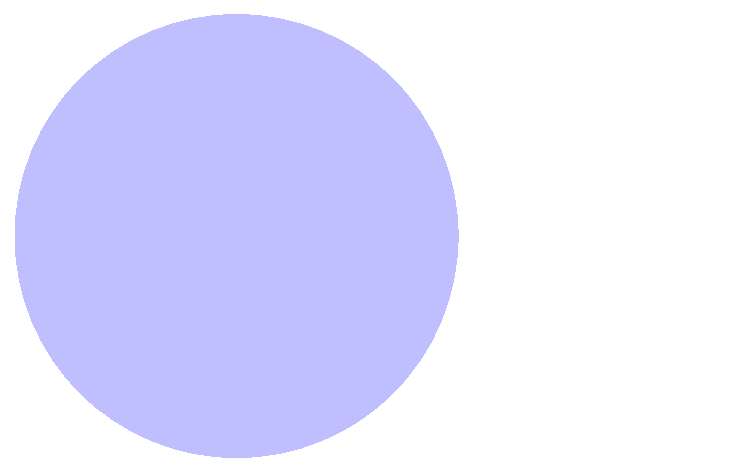
\includegraphics[ width = 1.25in ]{graphics/"monte carlo"/A}} &
    detected photons \\[15pt]
  %
    B &
    \raisebox{-0.5\height}{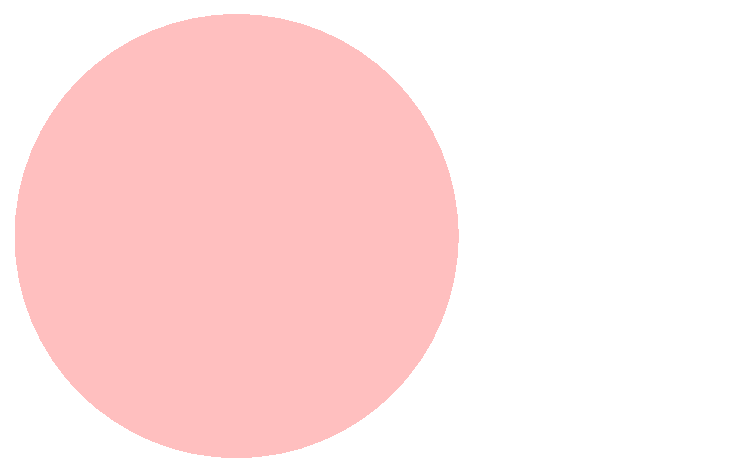
\includegraphics[ width = 1.25in ]{graphics/"monte carlo"/B}} &
    expected photons \\[15pt]
  %
    A $+$ B &
    \raisebox{-0.5\height}{\includegraphics[ width = 1.25in ]{graphics/"monte carlo"/"A + B"}} &
    ??? \\[15pt]
  %
    A $-$ B &
    \raisebox{-0.5\height}{\includegraphics[ width = 1.25in ]{graphics/"monte carlo"/"A - B"}} &
    photons scattered in \\[15pt]
  %
    B $-$ A &
    \raisebox{-0.5\height}{\includegraphics[ width = 1.25in ]{graphics/"monte carlo"/"B - A"}} &
    photons scattered out \\[15pt]
  %
    A $\cap$ B &
    \raisebox{-0.5\height}{\includegraphics[ width = 1.25in ]{graphics/"monte carlo"/"A int B"}} &
    unscattered photons \\[15pt]
  %
\end{tabular}
\end{center}
\label{tab:Venn}
\end{table}%


\endinput %-------------------------------